%!TEX root = ../dissertation.tex
\chapter{Preface}
\label{introduction}

Dear Reader! 

I am glad you are reading this dissertation.  

Writing the dissertation is not an easy task. I have to summarize six years of my professional life into about two hundred pages, so let me start by presenting the scope of my Ph.D. project. 

All of my activities during the doctoral studies were related to one of four biggest, currently operating experiments at  The European Organization for Nuclear Research CERN (fr.  Organisation européenne pour la recherche nucléaire).  It is called LHCb and it stands for Large Hadron Collider beauty experiment. The crucial part of the experiment is LHCb detector. The figure \ref{fig:LHCBphoto} presents the photo of the LHCb detector. Since there is not much to see beside the support steel structures I also added a schematic cross section of the experimental setup in Figure \ref{fig:}


\begin{figure}
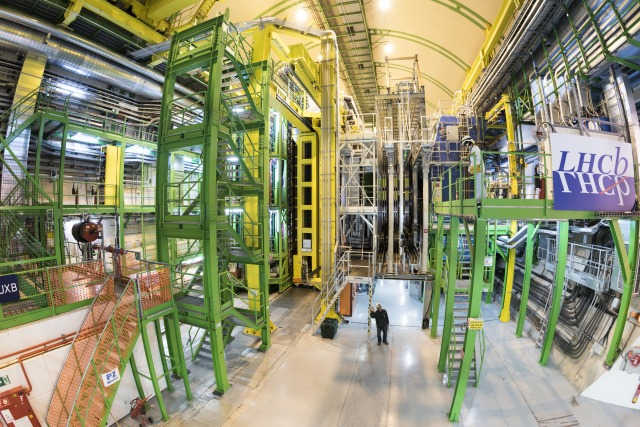
\includegraphics[width=\textwidth]{figures/LHCB_photo}
\caption{View of the detector LHCb. The image was taken from the CERN public website. 
\label{fig:LHCBphoto}}
\end{figure}

\begin{figure}
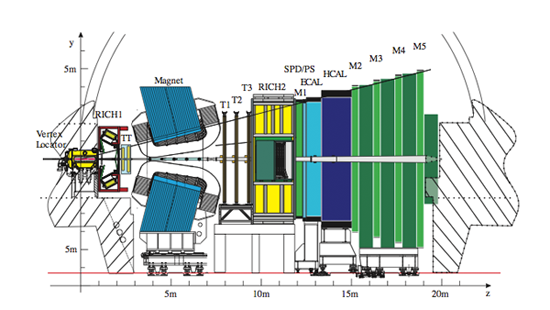
\includegraphics[width=\textwidth]{figures/lhcblayout.png}
\caption{Layout of the LHCb detector, viewed from the side. The LHCb detector components from left to right: proton-proton interaction point, Vertex Locator Velo, Ring Imaging Cherenkov detector one (RICH1), TT, Magnet, T stations, RICH2, electromagnetic and hadrinic calorimeter (ECAL and HCAL), and muon stations. Figure taken from \cite{lhcb_layout}. 
\label{fig:LHCBlayout}}
\end{figure}


As you may notice, the LHCb is a single-arm forward spectrometer. It was designed to cover the pseudorapidity range $2< \eta < 5 $  \cite{LHCb_TDR}. The pseudirapidity is a spatial coordinate describing the angle of a particle relative to the beam axis. The  pseudorapidity can be calculated using the following formula: 

\begin{equation}
    \eta = - \ln\left[ \tan \left( \frac{\vartheta }{2}\right) \right]\nonumber = \frac{1}{2} \ln \left( \frac{|\vec{p}|+ p_t}{|\vec{p}|- p_t}  \right)
    \label{eta}
\end{equation}

where: $\vartheta$  is the angle between the particle three-momentum $\vec{p}$ and the positive direction of the beam axis. The $p_t$ (transverse momentum) is a component of the $\vec{p}$ transverse to the beam line.

The equation \ref{eta} allows us to find the relationship between the parameter $\eta$ and the angle $\vartheta$. When the angle $\vartheta$ is getting smaller, then the $\eta$ is raising.    

From the physics point of view, the LHCb physics programme is primary focused on studying CP violation and rare phenomena in B (beauty) and C (charm) meson decays, and searching for New Physics. 
The high quality physics results obtained during the LHC Run 1 and Run 2 shows, proved excellent performance of the detector.
The list of outstanding physics results published by the LHCb Collaboration is extraordinary. 
For instance, the very first observation of the pentaquarks, or observation of the doubly charmed baryon  $\Xi_{cc}^{++}$.   
Although, no physics phenomena beyond the Standard Model have been found. Since no other heavy particle were discovered, apart from the Higgs boson, in general purpose experiments the precision studies may be the only way to detect the new effects at LHC. To be able to make that kind of analysis the LHCb Collaboration needs to collect as large as possible data samples data delivered by LHC. 

I would like to make shortly discussion of the units, that are customarily used to quantify the amount of collected data in High Energy Physics experiments. 
The particle collider performance is quantified by the beam energy and the integrated luminosity. The luminosity is defined as  the ratio of the  number of events detected $N$ in a certain time $t$ to the interaction cross-section $\sigma$:  
\begin{equation}
    L = \frac{1}{\sigma} \frac{dN}{dt}
\end{equation}
In practice, the integrated luminosity $\mathcal{L}_{int}$ with respect to the time is used instead. Based on this quantity we can estimate the number of expected events for a given process. The plot \ref{fig:Luminosity} presents the luminosity delivered to all of the LHC experiments. We clearly see the current LHCb read-out and trigger systems limit the data that could be collected. This limitation comes from the detector's maximum read-out rate of 1.1 MHz. To read out the full detector at an increased event rate requires a notable change in the LHCb read-out architecture.  

The LHCb trigger system is split into two stages. The level 0 trigger (L0) implemented in hardware, followed by the high level trigger (HLT) fully implemented in software which runs on a dedicated computing farm (Event Filter Farm) consisting of approximately 29 000 cores. 
The main task of the L0 trigger is to reduce the rate of visible interactions  from approximately 13 MHz to 1.1 MHz at which the full detector can be read out.  To achieve this goal a decision has to be reached by the hardware system within a fixed time of 4 μs. The L0 decisions are based exclusively on information from the muon system and calorimeters,  as these are the only pieces of information available in LHCb spectrometer at LHC clock  rate (40 MHz). Events  with  either  high $p_T$ muons  or  large  transverse  energy  deposits  in  the calorimeter are selected by L0.


\begin{figure}
\centering
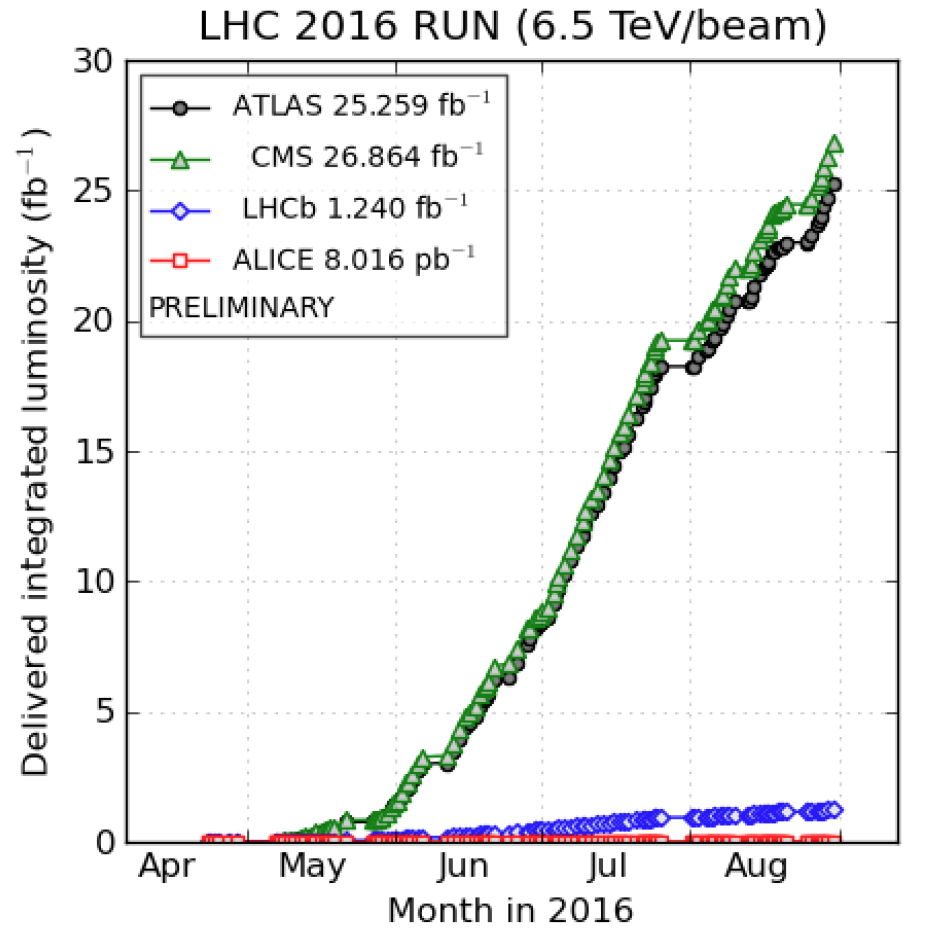
\includegraphics[scale=0.3]{figures/Luminosity.png}
\caption[Luminosity]{The integrated luminosity delivered to LHC experiments
\label{fig:Luminosity}}
\end{figure}

The key part of the Upgrade project is the replacement of the read-out system, which is currently limited by the Level-0 trigger to 1 MHz, to 40 MHz trigger system. This allows imputing of the full event to the LHCb acquisition farm and apply full software trigger for every bunch crossing. 
This goal can be achieved by replacing both read-out electronics and sensitive elements of the detectors. One of the most challenging parts of the Upgrade is research and development related to the design and test of the completely new tracking detector called Upstream Tracker. This silicon micro-strip detector will be placed just before the bending magnet and it supposed to replace current TT tracker. The detailed description of the UT detector can found in the section??.  The motivation to replace the current TT detector is motivated by three facts. First of all, the TT design doesn’t allow to survive expected radiation damage, in particular in the inner, close to the proton beam region. Secondly, the current sensors granularity could lead to an unaccepably high occupancies under the foreseen running conditions. Furthermore, the front-end Beetle chip, which is an essential part of the read-out system, is not able to process the raw data at the beam crossing rate (40 MHz). What makes the situation even worse the front-end hybrides, which were designed to support the Beetle chip, are part of the mechanical structure of the detector and cannot be replaced without damaging them. In addition, the new detector is designed to improve the LHCb acceptance.  

I was personally involved in the activities connected to the testing and verification of the UT silicon sensors. I participated in the number of the Testbeam campaigns, I designed and implemented a complete emulation platform for the raw data processing and data analysis. What are and why do we need the Testbeams? 

The teastbeam plays the key role in the new detector R'\&D' process. It is important to quantify the performance of the various sensors that have been subjected to the maximal radiation dose expected for a given sensor during the whole lifetime of the UT detector. Furthermore, the Testbeams provide realistic testbeds to confirm the expected performance of the whole data readout chain including the front-end ASICs. During the Testbeams, we collected the data, which allowed us for instance to study Landau distribution as a function of the bias voltage, cluster sizes versus bias voltage and resolution vs angle. All of the mentioned studies were performed for both irradiated and unirradiated sensors. The detailed description of the analysis of the Testbeam data is a topic of the section ??.

Before, we could make any analysis of the Testbeam data we had to design and develop software for raw data processing. The package is called TbUT and its source code can be found here. I was the main developer, and the one who was responsible for the software maintenance. The software was a very good achievement. Its flexible design allows to process data collected by the various DAQ electronics (ref to alibava and mamba), during the entire R'\&D' phase. The detailed description of the TbUT framework is a subject of the Chapter 3. Furthermore, the software will be possibly use to monitor the performance of the UT raw data. It will be a crucial part of the future platform to detector calibration. 


Moreover, as a member of the LHCb collaboration, I was involved in an improvement of the Downstream Tracking algorithm. You will find a more detailed description of the tracking algorithm in Chapter 3. Briefly, the tracking is a procedure which is designed to reconstruct the trajectory of the particles that were created as a result of the proton-proton collisions. The reconstruction algorithm is executed in a real time, as part of the trigger procedure, therefore it has to be very fast. However, due to the number of particles created during each beam crossing the previous implementation of the tracking procedures often made mistakes. Those mistakes corresponds to reconstructions of the fake, also called the ghost, tracks. To avoid such situation we decided to leverage Machine Learning and Deep Learning techniques. Basically, I enhanced the tracking procedure by adding the Machine Learning classifier, which was trained to distinguish whether the partially reconstructed track is a true one or not. As far as I know, the LHCb is the only one currently operating High Energy Physics experiment, which make use of advanced Machine Learning models as a part of the online trigger. During the development I familiarized myself with the concept of how to build entire Machine Learning pipeline using such open-source tools as sklearn, XGBoost, PyTorch and Keras. Such a technologies are widely used in both academia and industry. If you want to know more about Machine Learning and the procedure, how to build and deploy the model, please take some time to read the second part of the Chapter 3. 


I hope you enjoy reading this thesis. 

